% Updated in September 2014 by Hideo Saito
% Updated in September 2012 by In Kyu Park
% Updated in April 2002 by Antje Endemann, ...., and in September 2010 by Reinhard Klette
% Based on CVPR 07 and LNCS style, with modifications by DAF, AZ and elle 2008, AA 2010, ACCV 2010, ACCV 2012

\documentclass[runningheads]{llncs}
\usepackage{graphicx}
\usepackage{amsmath,amssymb} % define this before the line numbering.
%\usepackage{lineno}
\usepackage{color}
\usepackage{cite}

%===========================================================
\begin{document}

%macro for raising the point in decimal numbers; see example in the abstract
\newcommand{\point}{
    \raise0.7ex\hbox{.}
    }

%Do   -- NOT --    use any additional macros

\pagestyle{headings}

\mainmatter

%===========================================================
\title{Camera Motion and Surrounding Scene Appearance as Context for Action Recognition} % Replace with your title

\titlerunning{Camera Motion and Scene Appearance as Context for Action Recognition} % Replace with your title

\authorrunning{Fabian Caba Heilbron, Ali Thabet, Juan Carlos Niebles, Bernard Ghanem} % Replace with your names

\author{Fabian Caba Heilbron\textsuperscript{1,2}, Ali Thabet\textsuperscript{1}, Juan Carlos Niebles\textsuperscript{2}, Bernard Ghanem\textsuperscript{1}} % Replace with your names
\institute{\textsuperscript{1}King Abdullah University of Science and Technology (KAUST), Saudi Arabia\\
\textsuperscript{2}Universidad del Norte, Colombia} % Replace with your institute's address

\maketitle

%===========================================================
\begin{abstract}
This paper describes a framework for recognizing human actions in videos by incorporating a new set of visual cues that represent the \emph{context} of the action. We develop a weak foreground-background segmentation approach in order to robustly extract not only foreground features that are focused on the actors, but also global camera motion and contextual scene information. Using dense point trajectories, our approach separates and describes the foreground motion from the background, represents the appearance of the extracted static background, and encodes the global camera motion that interestingly is shown to be discriminative for certain action classes. Our experiments on four challenging benchmarks (HMDB51, Hollywood2, Olympic Sports, and UCF50) show that our contextual features enable a significant performance improvement over state-of-the-art algorithms.
\end{abstract}

%===========================================================
\section{Introduction} \label{introduction}
Human action recognition is a challenging task for computer vision algorithms due to the large variabilities in video data caused by occlusions, camera motion, actor and scene appearances, among others. A popular current trend in action recognition methods relies on using local video descriptors to represent visual events in videos \cite{laptev2005, dollar2005, wang2011}. These features are usually aggregated into a compact representation, namely the bag-of-features (BoF) representation \cite{laptev2008}. The advantage of this simple representation is that it avoids difficult pre-processing steps such as motion segmentation and tracking. In the BoF representation, local descriptors are quantized using a pre-computed codebook of visual patterns. This representation combined with discriminative classifiers such as support vector machines (SVM), has been quite successful in recognizing human actions  in controlled scenarios \cite{blank2005, schuldt2004}. Due to its simplicity, BoF requires the use of strong, robust and informative features, which can be obtained reliably in such simplified scenarios.

However, recent efforts have been made to collect more realistic video datasets (\emph{e.g.} from movies and personal videos uploaded to video sharing websites  \cite{kuehne2011,  marszalek2009}), which are useful for evaluating human action recognition methods in more natural settings. In fact, these datasets represent a challenge for existing BoF-based methods due to dynamic backgrounds, variations in illumination and viewpoint, and camera motion among other visual nuisances that can severely affect recognition performance. To mitigate the effect of camera motion in describing the action of interest in a video, recent methods \cite{wang2013,wang2011} have proposed using dense point trajectories in a video. In fact, these trajectories can separate background from foreground using a simple camera motion model (\emph{i.e.} an affine or homography transform between consecutive frames). Such separation allows action recognition approaches to robustly extract and describe foreground motion, which is otherwise contaminated by camera motion and the background. Inspired by this work, our proposed method also makes use of these dense trajectories; however, we enlist a more general camera model (by estimating the fundamental matrix between video frames) that allows for a more reliable separation between foreground and background pixels, especially in non-planar cluttered scenes.

Unlike most other methods, we claim that the \emph{context} of a human action, namely global camera motion and static background appearance, can also be used to discriminate between certain human actions. These cues are considered as contextual features for an action, which would allow classification algorithms to mine the relationship between the human action and both the background scene as well as the camera motion. The appearance of the scene in which an action occurs can be helpful in recognizing the action, as validated by previous work in \cite{marszalek2009}. For example, a `cooking' action tends to occur indoors, while a `jogging' action usually exists outdoors. Interestingly, the manner in which the \emph{cameraman} records a particular action can also be indicative of the action. For example, camera zoom with minimal panning usually indicates an action that is spatially limited to a smaller physical space (\emph{e.g.} juggling balls), while significant panning is indicative of actions that require a much larger spatial support (\emph{e.g.} practicing long jump). Our proposed approach mines these two sources of contextual information, as well as, the separated foreground motion to describe and recognize an action. Figure \ref{fig:pull_figure} illustrates our claims.

% Figure 1.
\begin{figure*}[ht]
\begin{center}
%\fbox{\rule{0pt}{1in} \rule{0.9\linewidth}{0pt}}
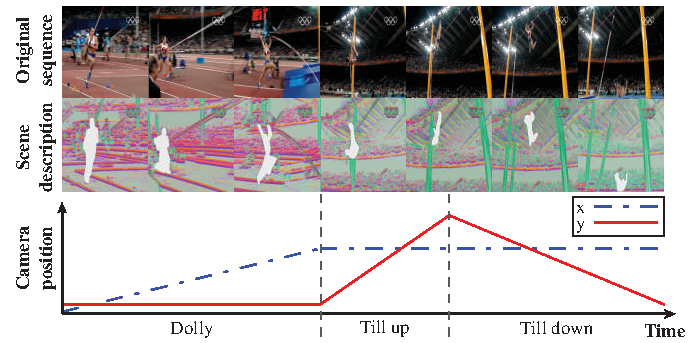
\includegraphics[width=0.98\linewidth]{pull_figure.pdf}
\end{center}
\vspace{-6pt}\caption{Some human actions have important correlations with surrounding cues. As observed in the first row, there is a video sequence associated with the human action pole vault. It is also noticeable that the camera moves according to some specific patron for capturing the movement of the subject. Specifically, the camera moves within dolly panning tracking when the athlete is approaching the plant and take off. Then, camera slightly starts to tilling up and tilling down when the person is flying away and falling respectively. Additionally, a better description can be performed if visual appearance of the track field is captured.}
\label{fig:pull_figure}
\end{figure*}


%-------------------------------------------------------------------------
% Related work
\subsection*{Related work}\label{subsec: related work}
A large body of work has studied the problem of human action recognition in video. For a survey of this work, we refer the reader to \cite{aggarwal2011}. In this section, we give an overview of previous work that is most relevant to our proposed method.

\paragraph{Action Recognition Pipeline.} The majority of action recognition methods rely on local descriptors to represent visual events in videos \cite{laptev2005,dollar2005,wang2011}. Traditionally, these features are usually aggregated into a compact representation using the bag-of-features (BoF) framework \cite{laptev2008, escorcia2013}. Moreover, recent studies show that using soft encoding techniques, such as  Fisher Vectors \cite{perronnin2010} and Vectors of Locally Aggregated Descriptors (VLAD) \cite{jegou2012}, can lead to a boost in action recognition performance. These representations combined with discriminative classifiers such as support vector machines (SVM), have been quite successful in discriminating human action classes. However, as discussed in \cite{xwang2013}, there remain many details of the overall action recognition pipeline that can be extensively explored, including feature extraction, feature pre-procesing, codebook generation, feature encoding and pooling and normalization. In this paper, we propose a new set of features that can be used to address some of the limitations of conventional feature extraction methods.

\paragraph{Feature Extraction.} When applied to videos with substantial camera motion, traditional feature extraction approaches \cite{dollar2005, laptev2005} tend to generate a large number of features, which are inherently dependent on the camera motion in a video, thus, limiting their discriminative power among action classes. In order to overcome this issue, Wu \emph{et al.} \cite{wu2011} propose the use of Lagrangian point trajectories for action description in videos captured  by moving cameras. Their method compensates for global camera motion by only extracting features that exhibit motion that is independent of the camera motion, thus, outperforming traditional feature extraction algorithms. In \cite{GhanemICPR2012}, these trajectories are used to recognize human actions using Fisher Kernel features for discrimination. Park \emph{et al.} \cite{park2013} use a weak video stabilization method based on extracting coarse optical flow to isolate limb motion while canceling pedestrian translation and camera motion. Wang \emph{et al.} \cite{wang2011} present a method for action recognition using dense sampling of point trajectories. Their method handles large camera motions by limiting the maximum length of tracked trajectories. Despite their simplicity, these dense trajectory features have been shown to achieve a significant performance improvement as compared to conventional spatiotemporal point features \cite{laptev2005}.

More recent methods improve upon the aforementioned dense trajectory features. For example, Jain \emph{et al.} \cite{jain2013} propose a method to estimate more reliable trajectory features for action recognition. This method lends additional reliability and robustness to trajectory extraction by decomposing optical flow into dominant and residual motions. Dominant motion is estimated using an affine frame-to-frame motion model and is subtracted from the computed optical flow to obtain the residual motion, which is attributed to the human action of interest. Similarly, `improved trajectories' are proposed in \cite{wang2013} to stabilize features and compensate for simple camera motion. This is done by fitting a frame-to-frame homography (using RANSAC) to separate moving points of the human action from those of the background. By explicitly canceling out the camera motion, their framework improves the performance of several motion descriptors, including trajectory shape, histogram of optical flow (HOF), and motion boundary histograms (MBH). While these methods have been successful in separating background and residual motions, contextual cues of actions are usually discarded, thus, ignoring relevant information such as static scene appearance and distinctive camera motions correlated with some actions.

Moreover, a few approaches have investigated ways to involve background scene information in the action recognition pipeline. Marszalek \emph{et al.} \cite{marszalek2009} incorporate context information from movie scripts by modeling the relationship between human actions and static scenes based on textual co-occurrence. While such textual co-occurrence helps recognition, they are restricted only to video sources where scripts are available. In \cite{ikizler2010}, multiple feature channels are integrated from different sources of information including human motion, scene information, and objects in the scene. However, this approach makes use of all pixels (corresponding to both the human action and background scene) to generate a global descriptor of the static scene \cite{oliva2001}. Rather than computing a holistic representation, our proposed method computes a static scene descriptor only from the extracted background, a motion descriptor from the extracted foreground trajectories, and a camera motion descriptor from the estimated transformations between consecutive frames.

In this paper, our goal is to reliably alleviate the effect of camera motion, as well as, incorporate features describing the surrounding of an action to build a richer representation for human actions. We are motivated by the fact that most videos are filmed with an intention and therefore there exists a correlation between the inherent camera motion in a video and the portrayed human action itself. We encode this intention with a weak camera motion model based on frame-to-frame fundamental matrices in a video. To the best of our knowledge, this is the first work to mine such a relationship between human actions and the filming process.

%===========================================================
\section{Proposed Methodology} \label{methodology}

% Figure 2
\begin{figure*}[t!]
\begin{center}
%\fbox{\rule{0pt}{3in} \rule{0.9\linewidth}{0pt}}
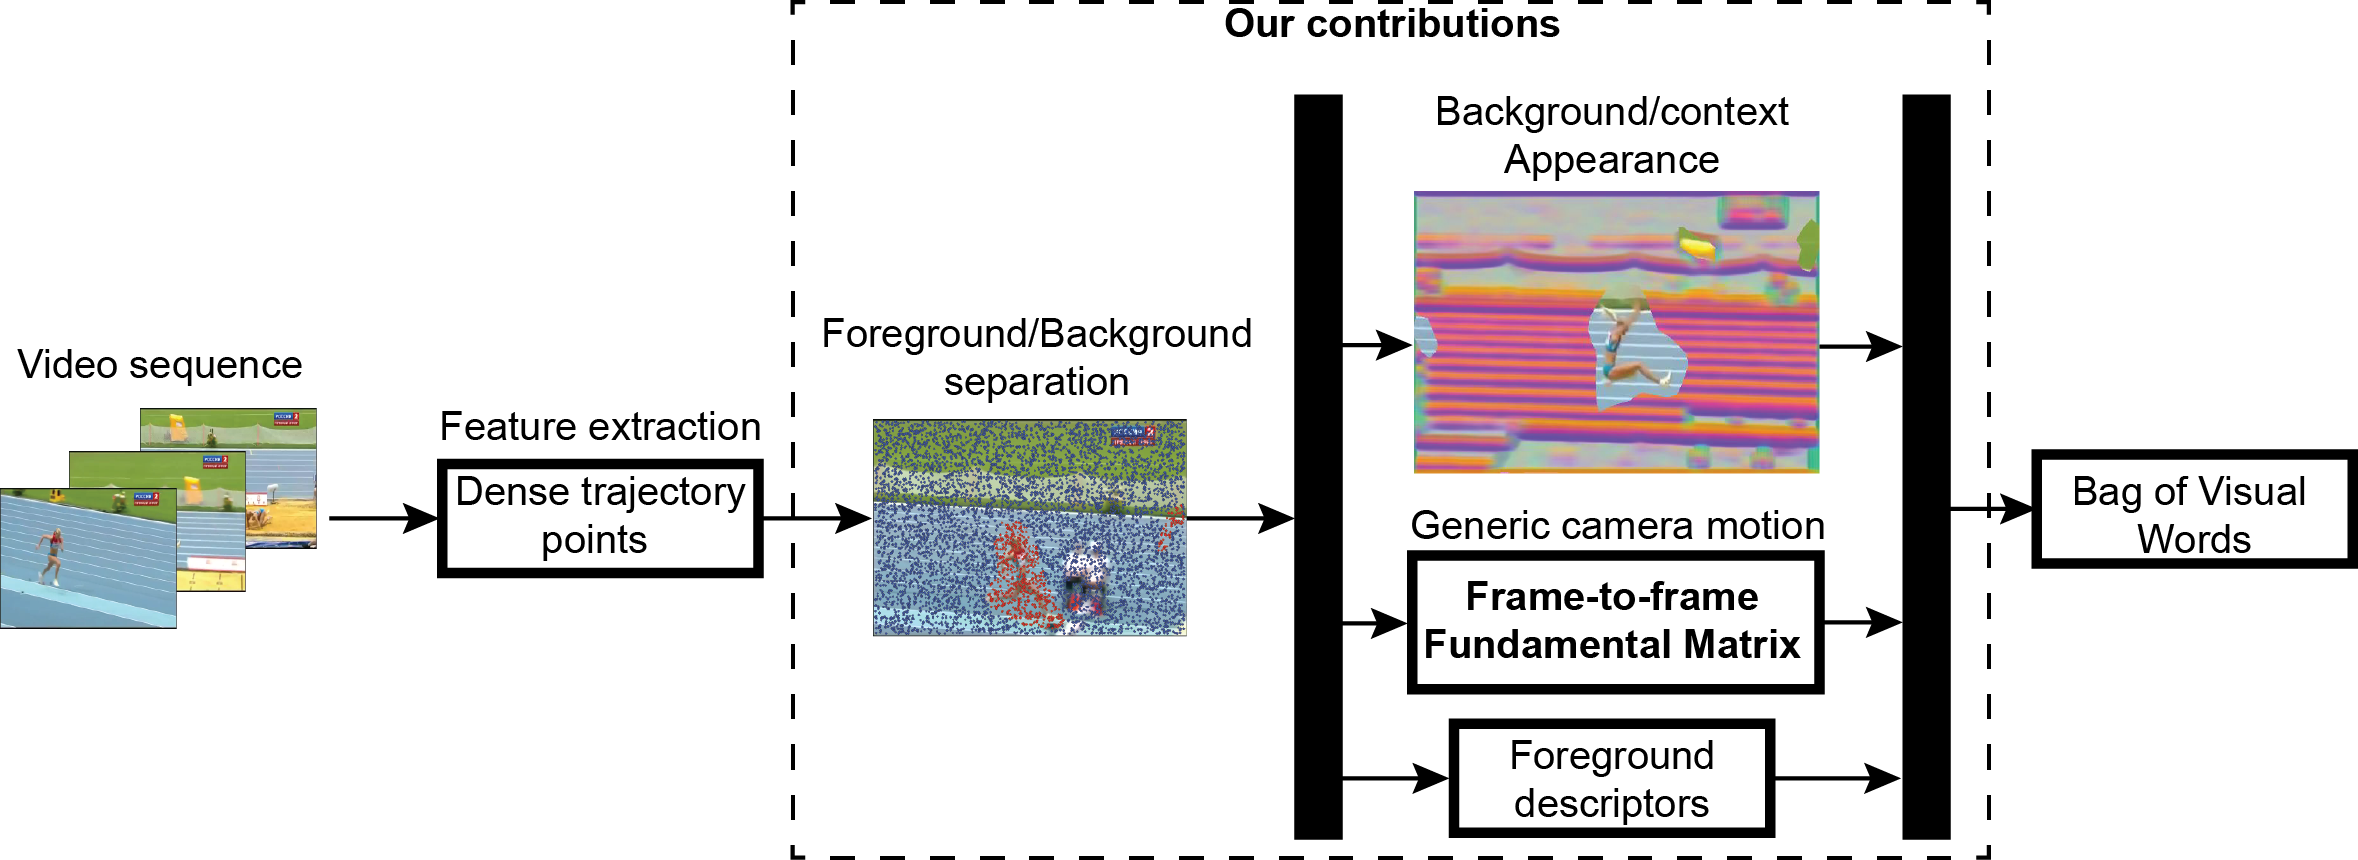
\includegraphics[width=0.98\linewidth]{pipeline.png}
\end{center}
\vspace{-12pt}\caption{Given a video sequence, a set of dense point trajectories are extracted. Then, a fundamental matrix is estimated and used to compensate for camera motion and to separate foreground from background trajectories. Each type of trajectories is encoded by a different descriptor. Specifically, frame-to-frame fundamental matrices are used to describe the camera motion. Moreover, surrounding scene appearance is explicitly computed on background trajectories. Traditional foreground descriptors (\emph{e.g.} MBH, HOF, HOG and trajectory shape) are also aggregated in action description. Finally, this set of descriptors is encoded separately using the BoF framework.}
\label{fig:pipeline}\vspace{-6pt}
\end{figure*}

This section gives a detailed description of our proposed approach for action recognition in video. The methodology in this paper follows the conventional action recognition pipeline. Given a set of labelled videos, a set of features is extracted from each video, represented using visual descriptors, and combined into a single video descriptor used to train a multi-class classifier for recognition.

In this paper, we use dense point trajectories (short tracks of a densely sampled set of pixels in a video \cite{wang2013}) as our primitive features. By estimating frame-to-frame camera motion (fundamental matrix), we separate foreground trajectories (corresponding to the action) from background ones. Each type of trajectory is represented using a different descriptor. Foreground trajectories are represented using conventional visual properties (\emph{e.g.} MBH, HOF, HOG, and trajectory shape), while the surrounding scene appearance is described using SIFT. Foreground and background trajectories are then encoded separately using the BoF framework as illustrated in Figure \ref{fig:pipeline}. Unlike other action recognition methods, we not only use the frame-to-frame camera motion to separate foreground from background, but we also use it to \emph{describe} a video. This is done by encoding all frame-to-frame fundamental matrices in a video using the BoF framework. We use all three descriptors (foreground, surrounding scene appearance, and camera motion) to train a multi-class classifier for recognition. In this paper, we argue and show that combining a foreground-only description \cite{wang2013} with additional cues (background/context and camera motion) provides a richer and more discriminative description of actions.


%-------------------------------------------------------------------------
\subsection{Camera Motion}
\label{subsec:cam_motion}
Since videos are normally filmed with the intention of maintaining the subject within the image frame, there exists a relationship between the estimated camera motion and the underlying action. In this paper, we argue and show that this relationship can be a useful cue for discriminating certain action classes. As observed in the three top rows of Figure \ref{fig:camMotion_example}, there is a correlation between how the camera moves and the actor For example, in the second row, the cameraman performs a downward tilt to follow the diver's movement. Here, we do not claim that this cue is significant for all types of actions, since very similar camera motion can be shared among classes, as shown in Figure \ref{fig:camMotion_example} (last two rows). Instead of using a homography to encode camera motion, we estimate the more general fundamental matrix for each pair of frames in a video using the well-known 8-point algorithm \cite{eightpoint97}. As mentioned earlier, a homography is suitable when the camera is not translating or when the background is planar; however, it is not applicable in more complex or cluttered scenes.

\begin{figure*}[!ht]
\begin{center}
%\fbox{\rule{0pt}{3in} \rule{0.9\linewidth}{0pt}}
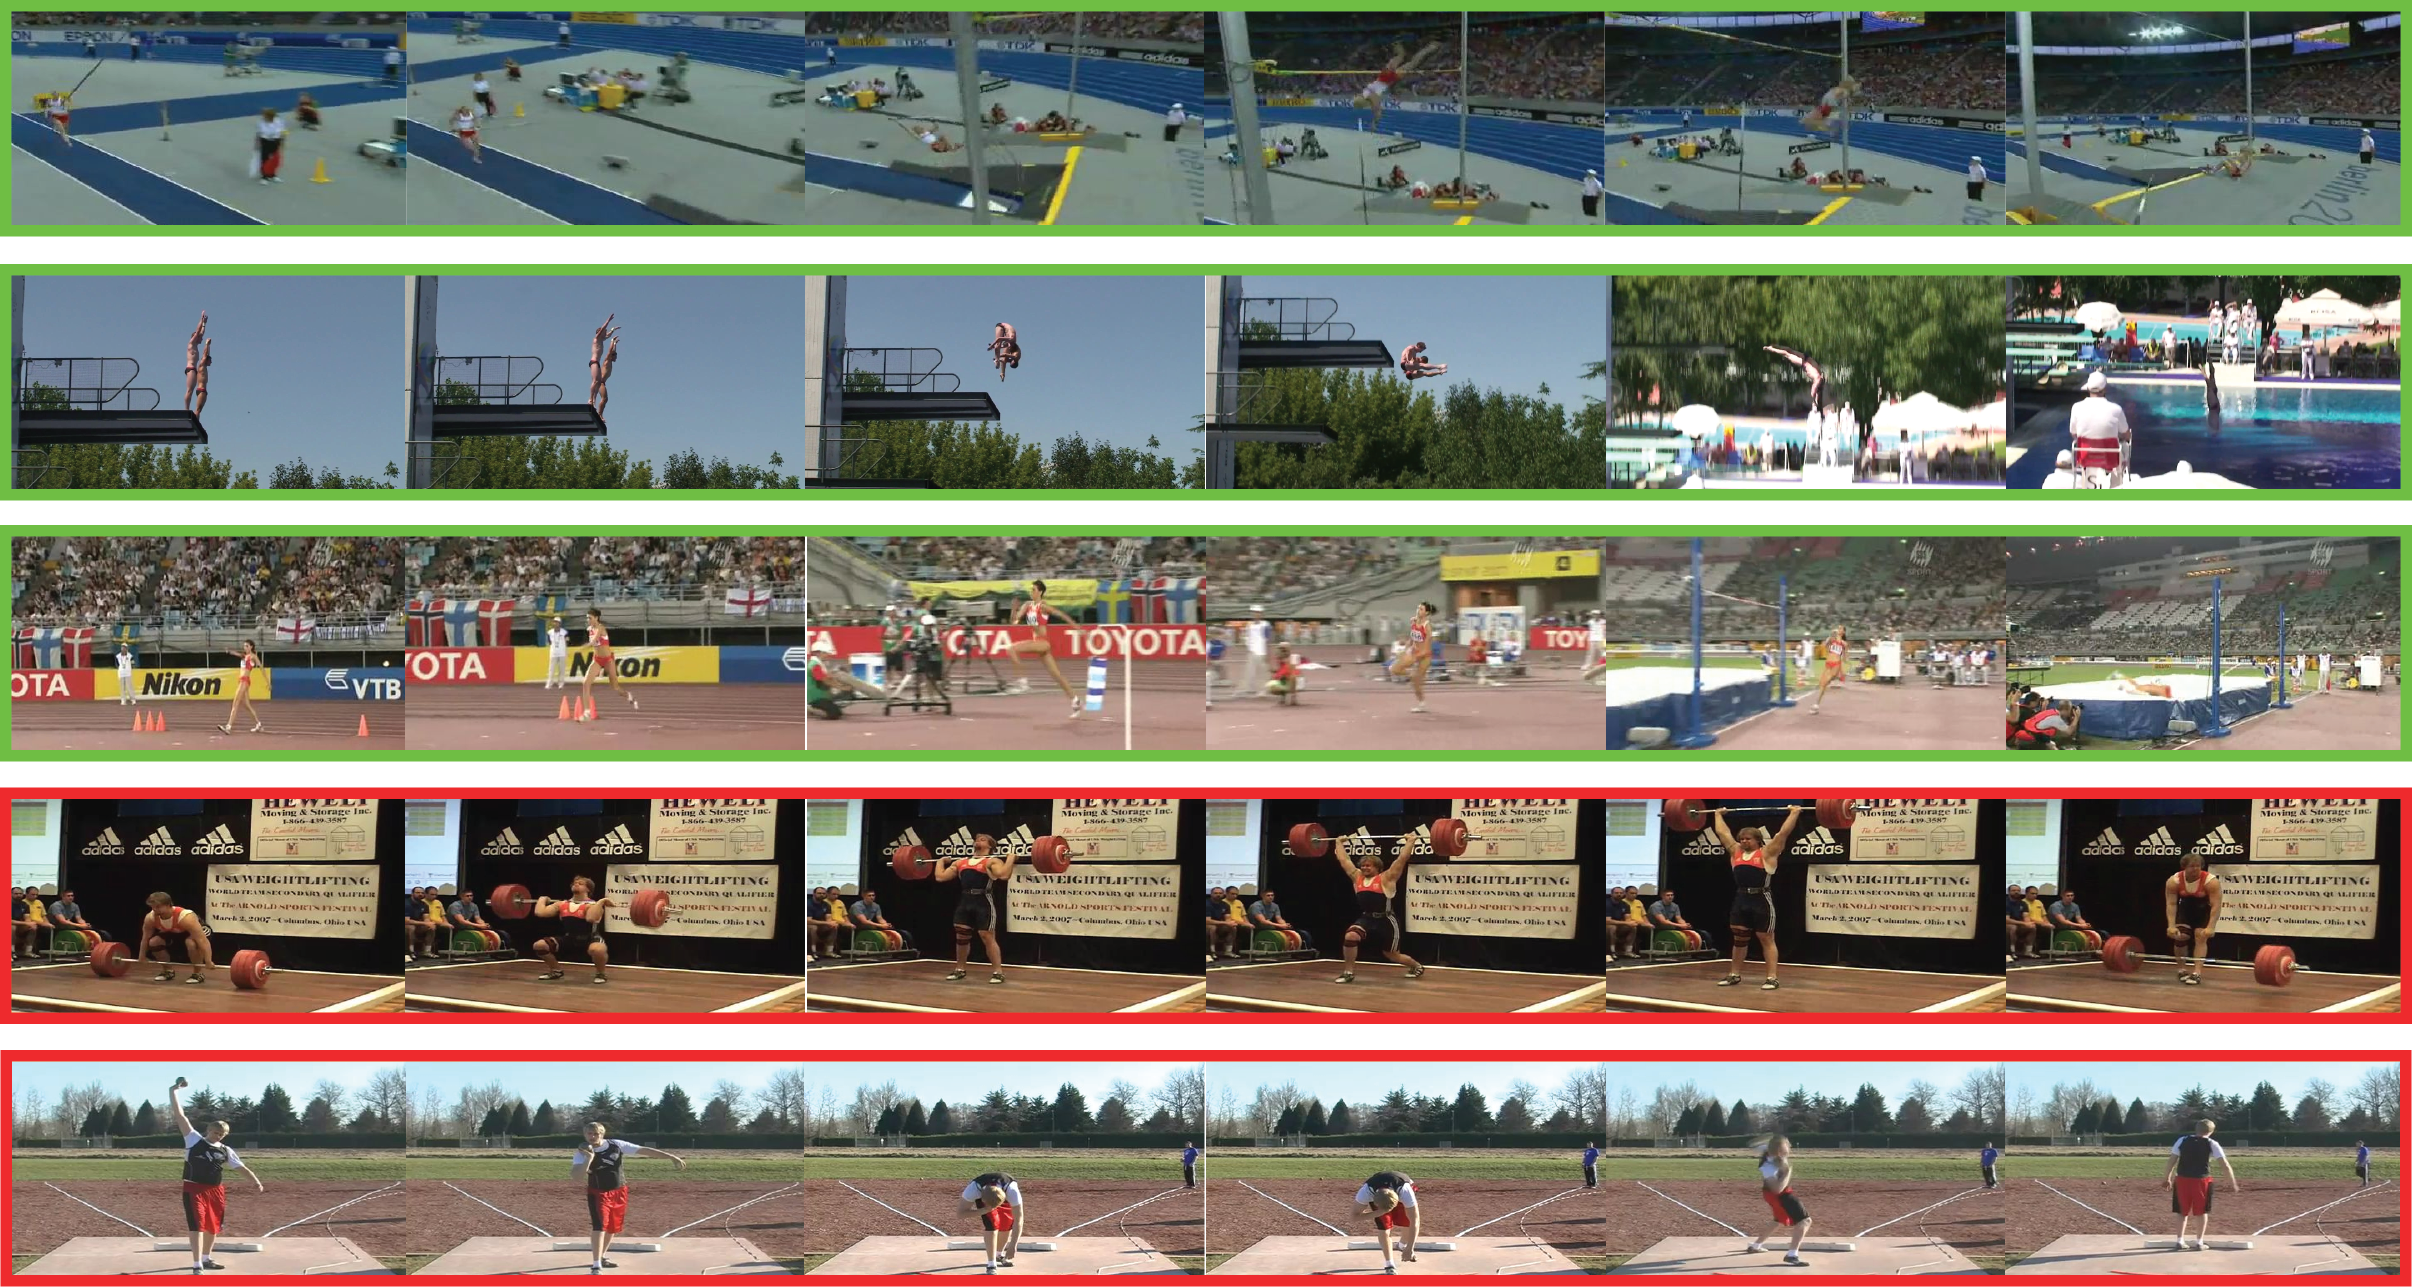
\includegraphics[width=0.98\linewidth]{cam_motion.png}
\end{center}
\vspace{-12pt}\caption{A generic camera motion descriptor can be a useful cue for discriminating specific action classes. The first three rows contain a characteristic correlation between how the camera moves and the action itself. However, this cue is not significant for all action classes, as exemplified in the last two rows, where there is no camera motion.}
\label{fig:camMotion_example}\vspace{-6pt}
\end{figure*}

In this paper, we compute the camera motion descriptor as follows. After estimating all pairwise fundamental matrices using RANSAC, we encode the camera motion of a video using the BoF framework. We call this descriptor CamMotion and it is complementary to other visual descriptors of the action. Unlike most existing work, we embrace camera motion and employ a low-level feature to represent it in a video.

\begin{figure*}[t!]
\begin{center}
%\fbox{\rule{0pt}{3in} \rule{0.9\linewidth}{0pt}}
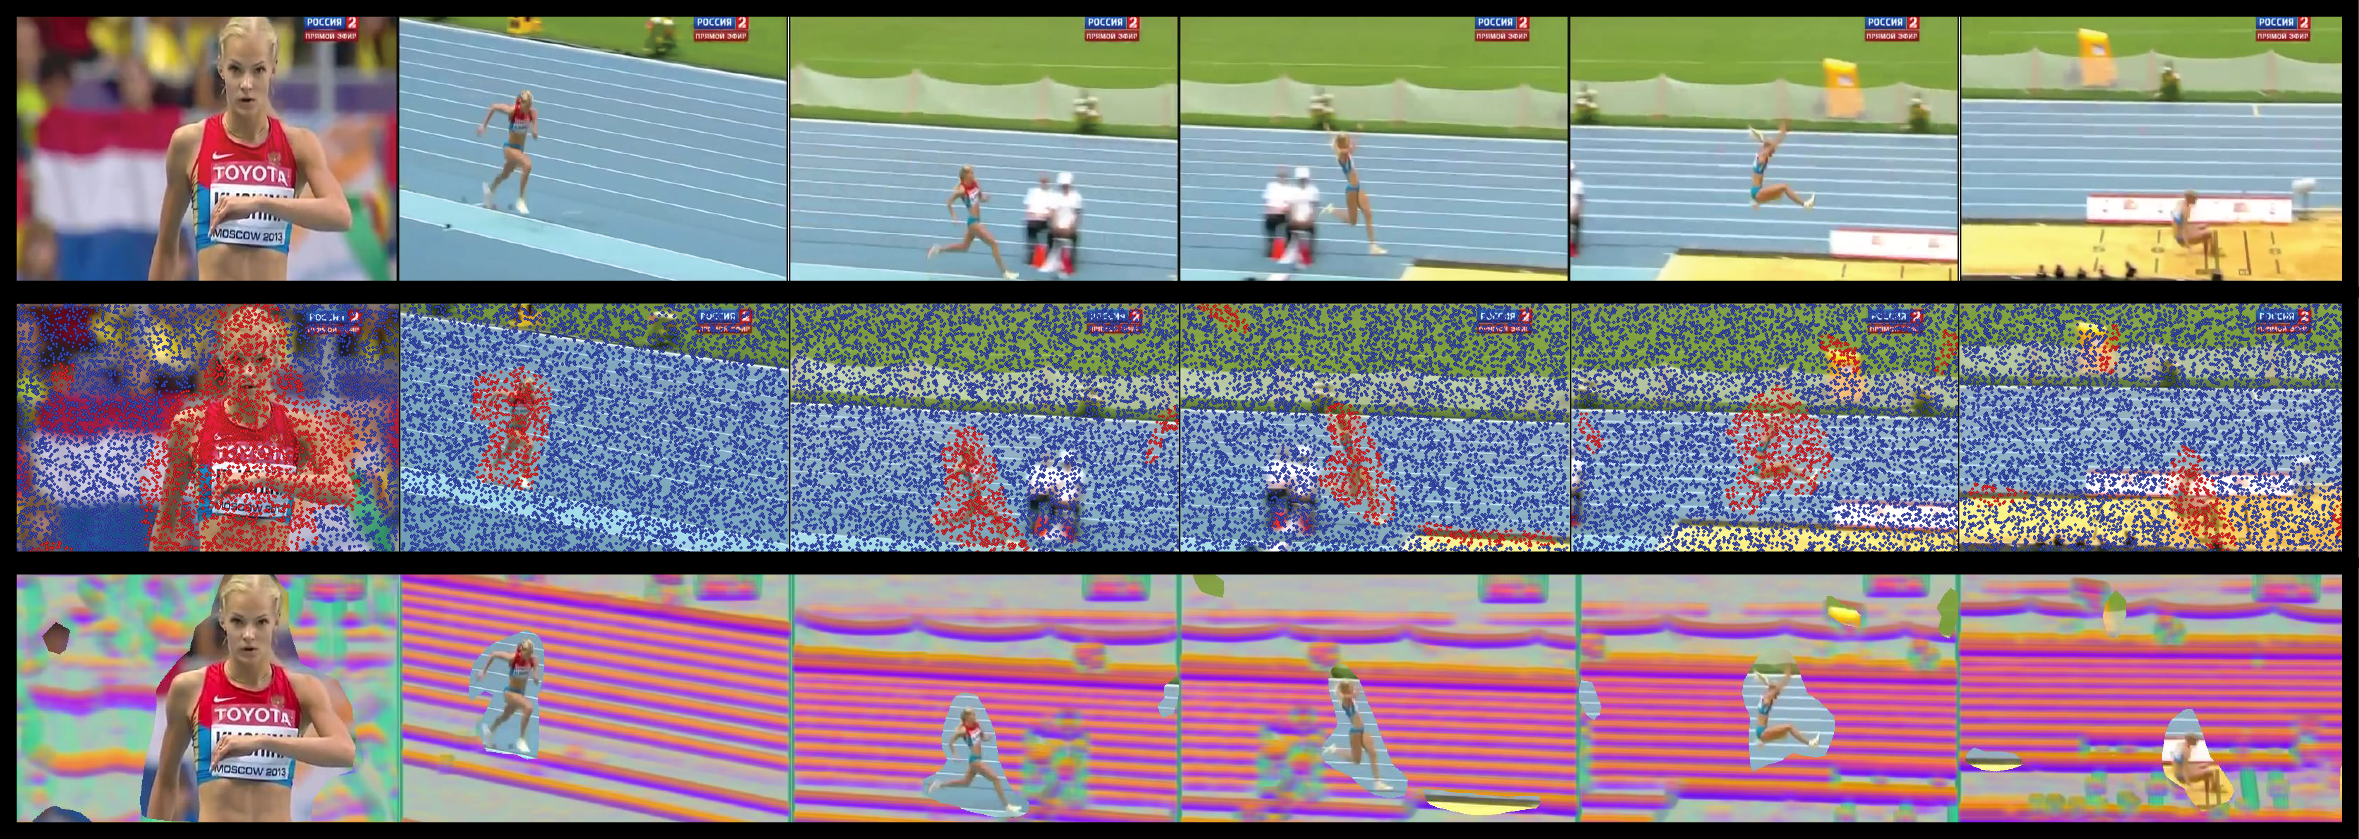
\includegraphics[width=0.98\linewidth]{approach.png}
\end{center}
\vspace{-6pt}\caption{Results from our foreground-background separation and illustration of the encoded information by the surrounding scene features. (\emph{top}) Frame sequence sampled from a 'long jump' video. Note that the camera is panning to follow the actor. (\emph{middle}) Camera compensation allows to perform a background-foreground separation. Noticeably, foreground feature points are mostly related with the actor. (\emph{bottom}) Illustration of information captured by our surrounding appearance SIFT descriptor. In order to achieve a meaningful illustration, descriptor dimensionality is reduced to 3 dimensions to produce a color-coded image. Surrounding appearance is represented using background points only, thus, avoiding confusion with pixels of the actor him/herself.}\label{fig:approach} \vspace{-6pt}
\end{figure*}


%-------------------------------------------------------------------------
\subsection{Foreground/Background Separation}\vspace{-2pt}
We use the global motion model introduced in Section \ref{subsec:cam_motion} to compensate for camera motion in the extracted point trajectories. To separate background from foreground, we assume that a background trajectory produces a small frame-to-frame trajectory displacement, after camera motion compensation. In fact, we simply threshold the overall displacement, which is computed for the $i^{\text{th}}$ trajectory as

\vspace{-6pt}
\begin{equation}
D(i) = \sum _{j=1}^{L-1}\left\|\mathbf{x}_{j+1}^i-\mathbf{x}_{j}^i\right\|_2^2.
\end{equation}
\vspace{-6pt}

Here, $\mathbf{x}_{j}^i$ represents the $j^{\text{th}}$ point in the $i^{\text{th}}$ trajectory. Trajectories are associated with the background if $D(i)\leq\alpha$; otherwise, they are labeled as foreground. Empirically, we set this threshold value to $\alpha=3$ pixels. Figure \ref{fig:approach} shows an example of our foreground-background separation in a video associated with the action \textit{long jump}. Here, foreground and background trajectories are color-coded in red and blue respectively. Clearly, the foreground trajectories correspond to the underlying action itself, while background trajectories correspond to \emph{static} background pixels undergoing camera motion only. Our proposed separation will allow each type of trajectory (foreground and background) to be represented independently and thus more reliably than other methods that encode context information using information from entire video frames \cite{marszalek2009}.

In this paper, we represent foreground trajectories using a foreground descriptor, comprising of Trajectory Shape, HOG, HOF, and MBH as in \cite{wang2013}. In the following section, we detail how surrounding scene appearance is encoded.



%-------------------------------------------------------------------------

\subsection{Background/Context Appearance}
Many visual cues can be used to discriminate human actions. Beyond local motion and appearance properties, the surrounding in which an action is performed is a critical component to recognize actions. For example, a 'springboard' action can only be executed if there is a pool, which has distinctive appearance properties. This motivates us to encode the visual appearance of the static scene. Surrounding scene appearance is encoded using SIFT descriptors \cite{lowe2004} around trajectory points associated with the background. We detect SIFT keypoints in a dense manner and then filter out those that fall within the union of foreground trajectories. Context appearance focuses more on the scene itself, as observed in Figure \ref{fig:sift_example}, where it can be used to aggregate meaningful information about the action. For example, all the examples of the action 'rowing' contain a shared scene appearance and layout which can be exploited to model the background trajectories. Unlike other methods that encode scene context holistically (using both foreground and background) in a video \cite{marszalek2009}, separating the background (or context) from the foreground produces a more reliable and robust context descriptor.



\begin{figure*}[t!]
\begin{center}
%\fbox{\rule{0pt}{3in} \rule{0.9\linewidth}{0pt}}
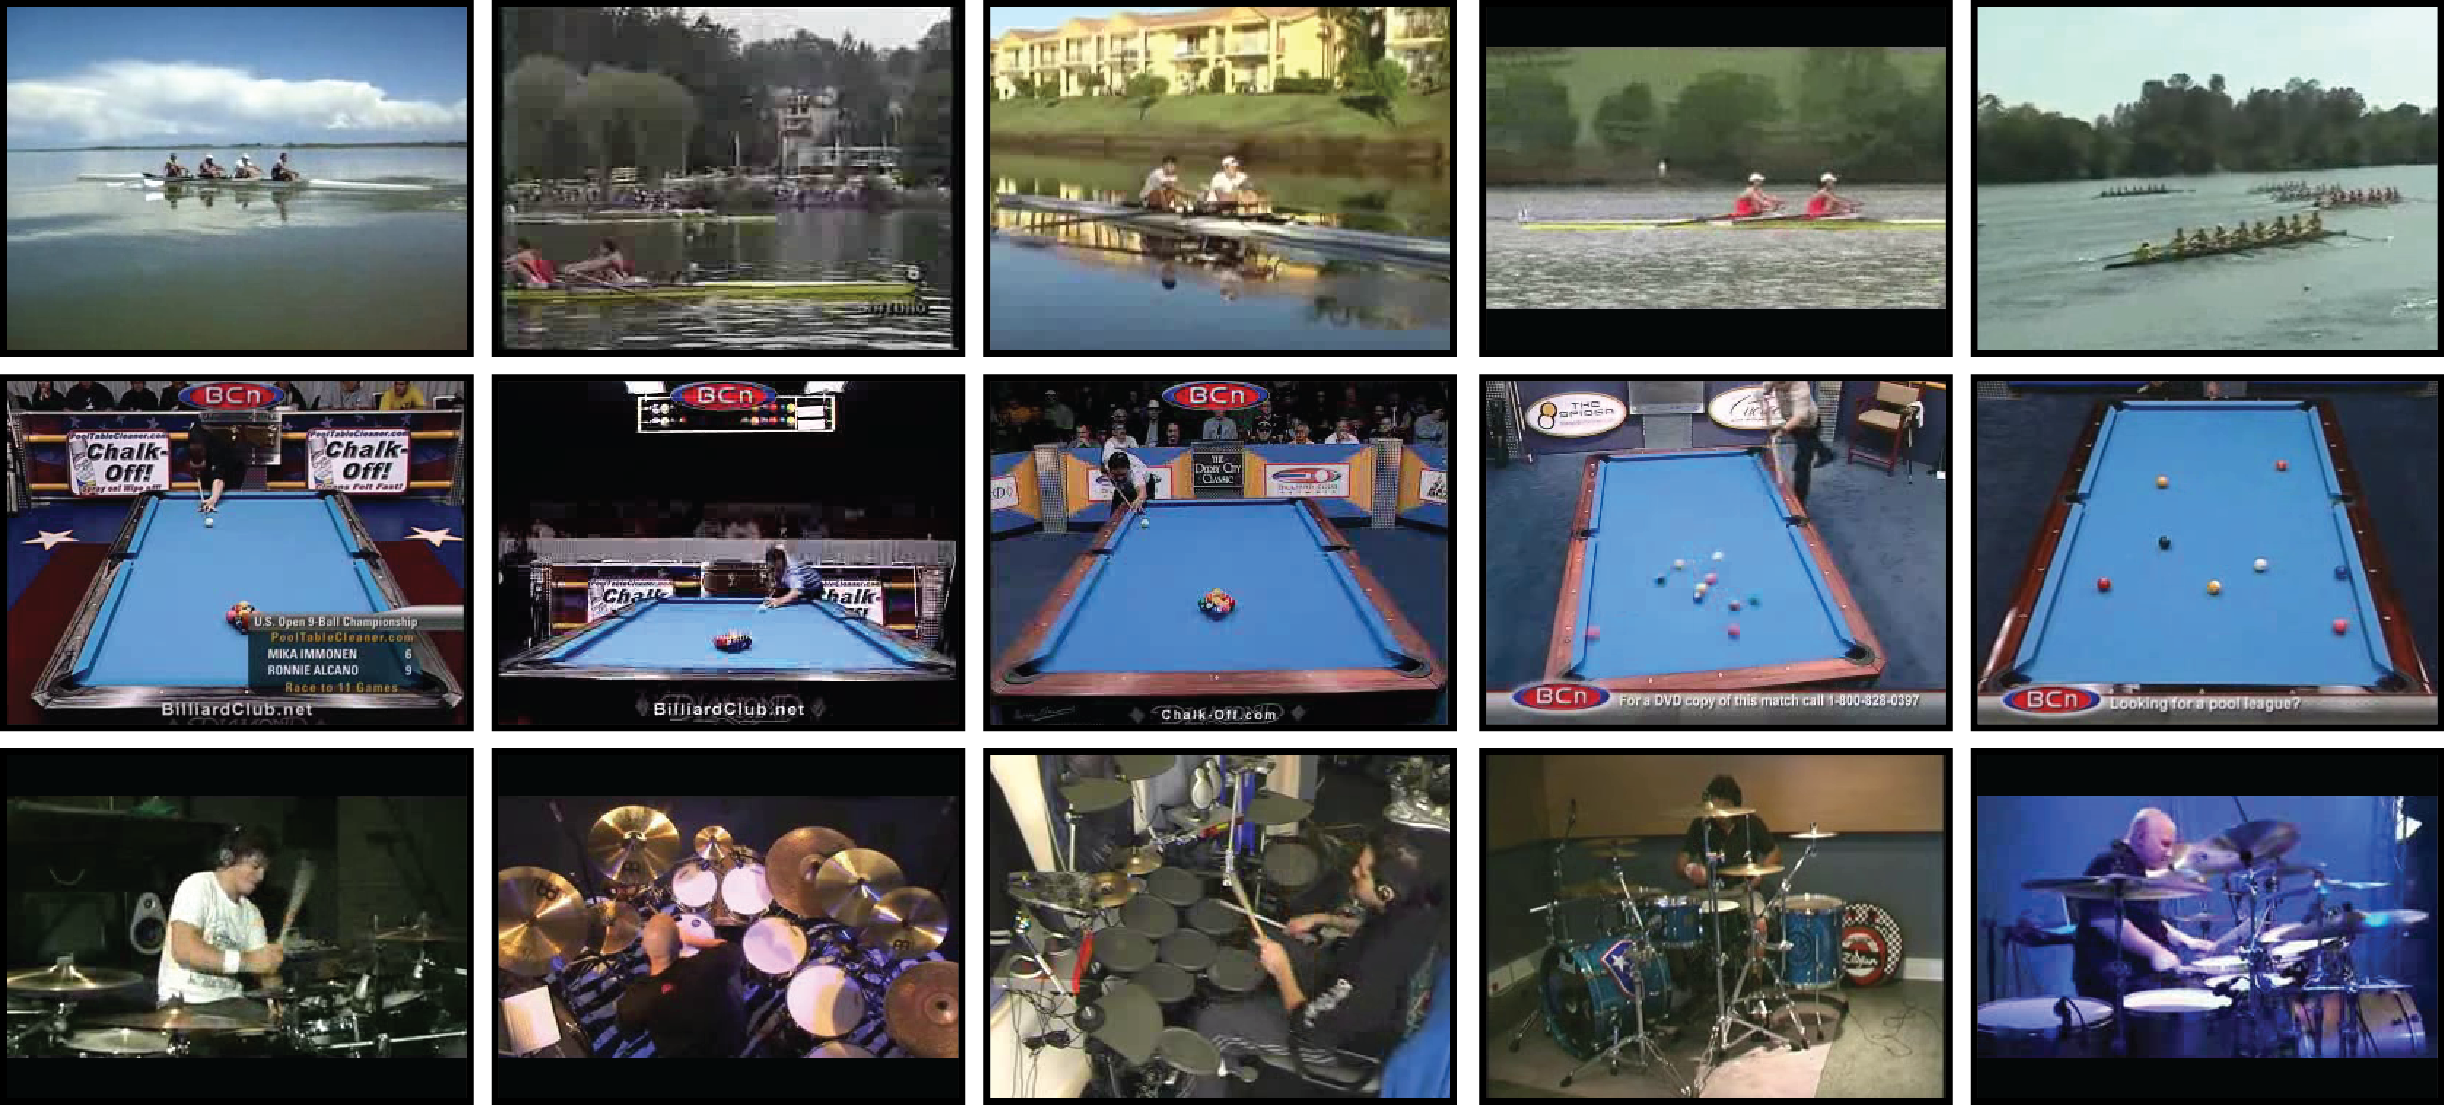
\includegraphics[width=0.98\linewidth]{sift.png}
\end{center}
\vspace{-6pt}\caption{Each row presents five different thumbnails taken from different videos of UCF50 dataset. (\emph{top}) Visual examples of the `rowing' action class. As observed all thumbnails share distinct background appearance \emph{i.e.} in all water is present and also in the majority there is a common landmark. (\emph{middle}) Visual examples of the 'billiard' action class. A billiard table and the indoor environment of the action, enable our surrounding appearance descriptor to capture critical information about that action. (\emph{bottom}) Visual examples of the 'drumming' class. Note that these examples share visual cues that are largely ignored if only foreground features are encoded.}
\label{fig:sift_example}
\end{figure*}

%%%%%%%%%%%%%%%%% Figure: Effect of sampling %%%%%%%%%%%%%%%%%%%
\begin{figure*}[t!]
\begin{center}
%\fbox{\rule{0pt}{1.2in} \rule{0.9\linewidth}{0pt}}
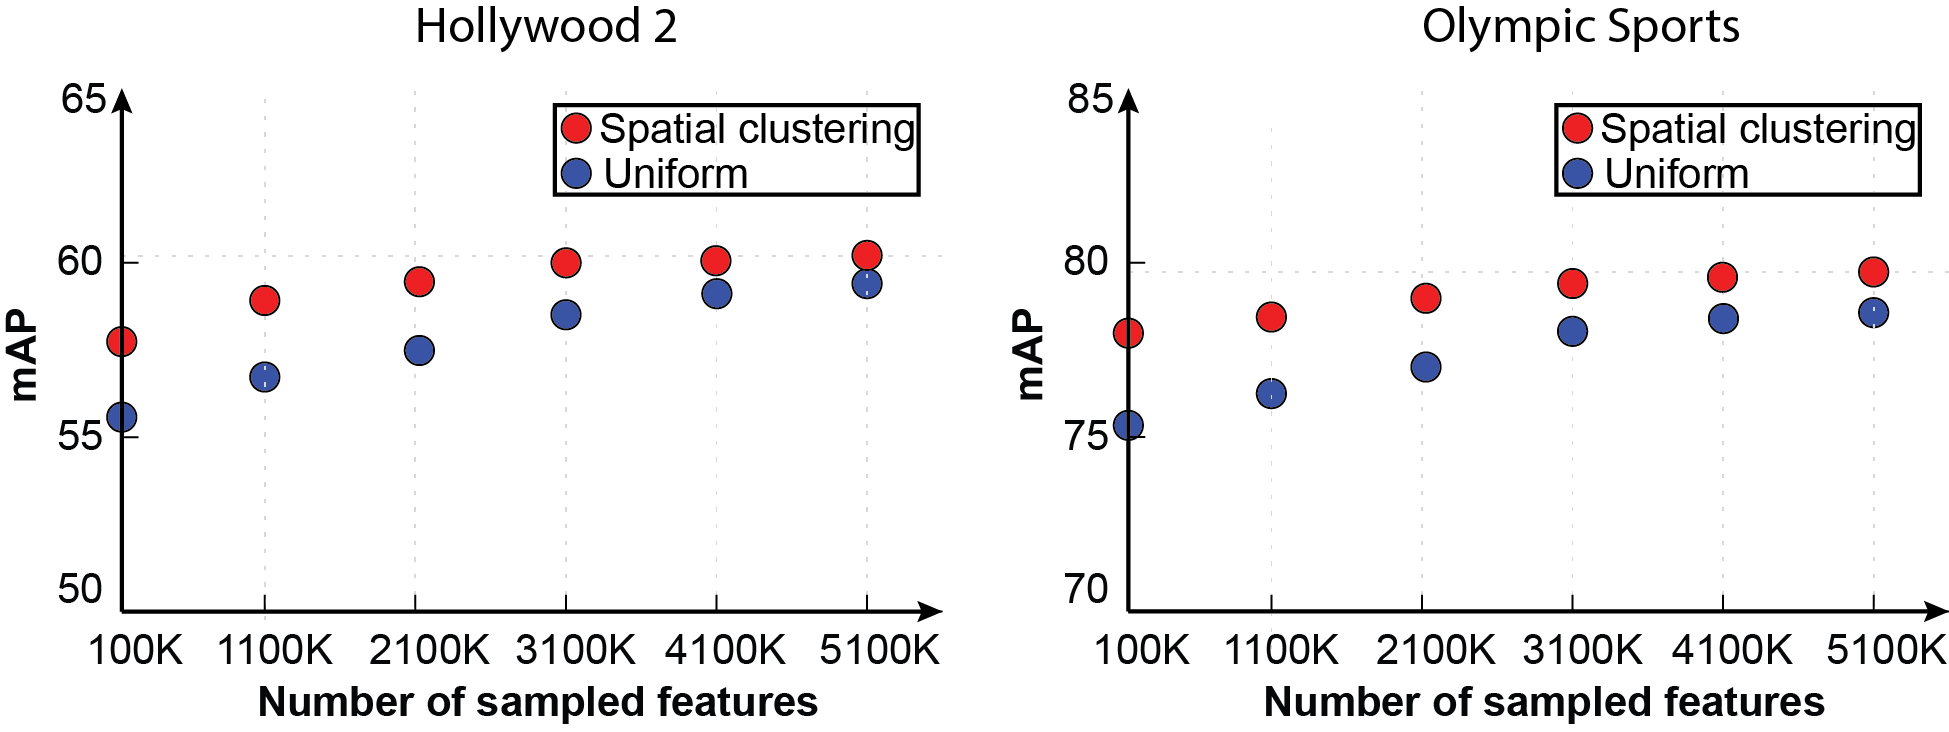
\includegraphics[width=0.98\linewidth]{sampling.png}
\end{center}
\vspace{-6pt}\caption{Due to the large number of features extracted by the dense trajectory method, sub-sampling is required to generate a codebook. Here, we explore the effect of the number of sampled features on the overall performance. A comparison is done on two different datasets under the Bag-of-Features framework. Also, the performance of two different sampling strategies is reported: uniform and spatial clustering. As noticed, selecting more features to form the codebook and using the spatial clustering approach improve recognition performance in both datasets.}
\label{fig:feature_sampling}
\end{figure*}
%%%%%%%%%%%%%%%%%%%%%%%%%%%%%%%%%%%%%%%%%%%%%%%%%%%%%%%%%%%%%%%%



%-------------------------------------------------------------------------
\subsection{Implementation details}\label{subsec:implementation}
\paragraph{Codebook Generation.} We generate the visual codebook in two different ways: (a) using k-means clustering or (b) using a Gaussian Mixture Model (GMM), which captures a probability distribution for the feature space. In both cases, a codebook is computed for each descriptor (context appearance, foreground, and camera motion) separately. Since the trajectory extraction method produces a large number of features from the training videos resulting in intractable codebook computation, it is necessary to sub-sample these features. In order to establish a trade-off between computation cost and recognition performance, we study the effect of the number of sampled features for computing a visual codebook, as observed in Figure \ref{fig:feature_sampling}. This experiment includes results on two different datasets using k-means clustering to form the visual dictionary. Moreover, we investigate two types of sub-sampling strategies, namely uniform random sampling and random sampling based on spatially clustered (using simple distance thresholding) trajectories. Based on results in Figure \ref{fig:feature_sampling}, the latter strategy outperforms the former one, especially when a small number of features are sampled. Therefore, in our experiments, we generate the visual codebook from 5 million feature points (~8GB RAM required per descriptor) sampled by the spatial clustering strategy.

\paragraph{Representation and Classification.} Feature encoding can be performed using one of two popular approaches: (a) traditional histogram quantization (VQ), or (b) Fisher vectors introduced in \cite{perronnin2010}. Different types of normalization are performed to provide robustness to feature vectors: (a) \textit{l2} normalization (L2) \cite{perronnin2010}, (b) power normalization (PW) \cite{perronnin2010}, and (c) intra-normalization (IN) \cite{xwang2013}. In our experiments, we focus on two classification frameworks that have been widely adopted in the action recognition literature. For simplicity, we summarize the details of each framework in Table \ref{tab:frameworks}. The first follows the Bag of Features (BoF) paradigm, using k-means for visual codebook generation, VQ for feature encoding, L2 normalization, and a $\chi^2$ kernel SVM within a multichannel approach (MCSVM) \cite{zhang2007}. In this case, the kernel is defined as

\begin{equation}
K(\mathbf{x}_i,\mathbf{x}_j)= \exp\left(-\sum_c {\frac{1}{2\Omega_c} D_c(\mathbf{x}_i,\mathbf{x}_j)}\right),
\label{eq:multichannel}
\end{equation}

\noindent where $D_c(\mathbf{x}_i,\mathbf{x}_j)$ is the $\chi^2$ distance for channel $c$ and $\Omega_c$ is the average channel distance. For the second framework, we enlist a more robust feature encoding scheme (Fisher vectors) using a visual codebook generated by learning a GMM on the subsampled training data. Here, each action video is represented as a high dimensional Fisher vector that undergoes three normalization procedures, L2, PW and IN as in \cite{xwang2013}. The three normalized features channels are concatenated and discriminative action models are learned using a linear SVM (LSVM).




%%%%%%%%%%%%%%% Table: Frameworks comparison %%%%%%%%%%%%%%%%%%%
\begin{table*}[h!]
\caption{Comparison of adopted frameworks for action recognition.}
\begin{center}
{
\begin{tabular}{ l| c c c c c }
\hline
Representation $\downarrow$ & Codebook & Encoding & Normalization & Classifier \\
\hline
Bag of Features & \textit{k}-means & VQ & L2 & MCSVM \\
Fisher vectors & GMM & Fisher vectors & L2+PW+IN & LSVM \\
\hline
\end{tabular}
}
\end{center}
\label{tab:frameworks}
\end{table*}
%%%%%%%%%%%%%%%%%%%%%%%%%%%%%%%%%%%%%%%%%%%%%%%%%%%%%%%%%%%%%%%%

%===========================================================
\vspace{-12pt}
\section{Experimental results}\label{results}
In this section, we present extensive experimental results that validate our contextual features within the action recognition pipeline. We compare the performance of both classifications frameworks mentioned in Section \ref{subsec:implementation}, as well as, state-of-the-art recognition methods on benchmark datasets, when possible.

\subsection{Datasets and Evaluation Protocols}
\label{subsec:datasets}
We use four public datasets \cite{kuehne2011, marszalek2009, niebles2010, reddy2013} and their corresponding evaluation protocols. In this section, we briefly describe each dataset.

\paragraph{HMDB51} \cite{kuehne2011} includes a large collection of human activities categorized on 51 classes. It comprises 6766 videos from different media resources \emph{i.e.} digitized movies, public databases and user generated web video data. Since many of the videos contain undesired camera motions, the authors provide a stabilized version of the dataset. However, since we look at the camera motion as an informative cue, the pre-stabilized version of the dataset is used. To evaluate classification performance, we adopt the same protocol proposed by the authors, namely the mean accuracy under three fixed train/test splits of the data.

\paragraph{Hollywood2} \cite{marszalek2009} contains a large number of videos retrieved from 69 different Hollywood movies. It is divided into 12 categories including short actions such as 'Kiss', 'Answer Phone' and 'Stand Up'. This dataset remains one of the most challenging despite the small number of action classes. Change of camera view,  camera motion and unchoreographed execution introduces significant difficulty to the recognition task. To evaluate performance, we follow the authors' protocol, whereby videos are separated in two different sets: a training set of 823 videos and a testing set of 884 videos. We use training videos to learn our action models and then compute the mean average precision (mAP) over all action classes.

\paragraph{Olympic Sports} \cite{niebles2010} or \textbf\textit{{Olympic}} comprises a set of 783 sport related YouTube videos. This set of videos are semi-automatically labeled using Amazon Mechanical Turk. This dataset establish new challenges for recognition because the underlying action classes range from simple actions (\emph{e.g.} 'Kiss') to complex actions (\emph{e.g.} 'Hammer Throw'). All of these complex actions are related to olympic sports including actions like 'Long Jump', 'Pole Vault' and 'Javelin Throw'. As proposed by the authors, we measure performance by computing the mAP over all action classes.

\paragraph{UCF50} \cite{reddy2013} includes 6618 videos of 50 different human actions. This dataset presents several recognition challenges due to large variations in camera motion, cluttered background, viewpoint, etc. Action classes are grouped into 25 sets, where each set consists of more than 4 action clips. Recognition performance is measured by applying a leave-one-group-out cross-validation and average accuracy over all group splits is reported.

\paragraph{UCF101} \cite{soomro2012} contains 13320 video clips within 101 different human action categories. This dataset is an extension of UCF50 (described above). We tightly follow the protocol outlined in the THUMOS 2013 action recognition challenge \cite{thumos2013}. 


%-----------------------------------------------------------
\subsection{Impact of Contextual Features}
In this section, we conduct experiments to evaluate the contribution of our proposed camera motion (CamMotion) and surrounding scene appearance descriptor (SIFT) to overall action recognition performance. Our baseline corresponds to using only Foreground features for describing actions. Using descriptors individually is compared to this baseline. Also, we investigate the effect of combining the proposed features with Foreground cues. As mentioned earlier, both action recognition frameworks (BoF and Fisher vectors) are explored. Below, we present an analysis of our obtained results.

\paragraph{Representation.} As suggested in recent works \cite{perronnin2010, wang2013, xwang2013}, Fisher vectors register an improved performance over traditional BoF representations. We found in our experiments that Fisher vectors also boost the performance of using our contextual descriptors. These results are reported in Table \ref{tab:features}. However, we note that using Fisher vectors is less important with our CamMotion descriptor due to its low dimensionality.

%%%%%%%%%%%%%% Table: Feature analysis %%%%%%%%%%%%%%%%%%%%%
\begin{table*}[ht!]
\caption{Impact of our surrounding scene appearance and camera motion features on recognition performance. Bag-of-Features encoding generally performs worse than Fisher vectors. Both surrounding SIFT and CamMotion show important improvements in performance when they are combined with foreground descriptors.}
\begin{center}
{
\def\arraystretch{1.11}
\setlength{\tabcolsep}{3.66pt}
\begin{tabular}{ |c c c|c c c c| }
\hline
\multicolumn{3}{|c|}{Features} & \multicolumn{4}{|c|}{Datasets} \\
Foreground & SIFT & CamMotion & HMDB51 & Hollywood2 & Olympics & UCF50 \\
\hline
\multicolumn{7}{|c|}{Framework: Bag of Features} \\
\hline
\checkmark & & & 51.2\% & 60.1\% & 79.8\% & 85.9\% \\
& \checkmark & & 19.5\% & 28.7\% & 36.4\% & 45.7\% \\
& & \checkmark & 13.5\% & 21.8\% & 26.9\% & 19.3\% \\
\checkmark & \checkmark & & 53.8\% & 60.9\% & 81.1\% & 87.2\% \\
\checkmark &  & \checkmark & 50.9\% & 60.4\% & 80.6\% & 86.8\% \\
& \checkmark & \checkmark & 20.7\% & 36.2\% & 43.7\% & 50.3\% \\
\checkmark & \checkmark & \checkmark & 51.7\% & 61.6\% & 81.7\% & 87.6\% \\
\hline
\multicolumn{7}{|c|}{Framework: Fisher vectors} \\
\hline
\checkmark & & & 56.5\% & 62.4\% & 90.4\% & 90.9\% \\
& \checkmark & & 20.1\% & 28.5\% & 39.6\% & 49.8\% \\
& & \checkmark & 14.1\% & 22.1\% & 27.2\% & 19.5\% \\
\checkmark & \checkmark & & \textbf{59.2\%} & \textbf{63.5\%} & \textbf{91.6\%} & \textbf{93.3\%} \\
\checkmark &  & \checkmark & 55.9\% & 62.9\% & 91.3\% & 93.1\% \\
& \checkmark & \checkmark & 22.3\% & 36.5\% & 46.5\% & 54.3\% \\
\checkmark & \checkmark & \checkmark & \textbf{57.9\%} & \textbf{64.1\%} & \textbf{92.5\%} & \textbf{93.8\%} \\
\hline
\end{tabular}
}
\end{center}
\label{tab:features}
\end{table*}
%%%%%%%%%%%%%%%%%%%%%%%%%%%%%%%%%%%%%%%%%%%%%%%%%%%%%%%%%%%%


\paragraph{Surrounding Appearance.} While the surrounding SIFT features achieves a discrete performance by itself, it also produces a notable improvement when combined with foreground descriptors. As Table \ref{tab:features} reports, performance is significantly improved over all datasets. Interestingly, we note that this features produces higher improvements in HMDB51 and UCF50.

\paragraph{Camera Motion.} Our experiments provide evidence that action recognition performance can be improved when global camera motion is incorporated with Foreground features. Our CamMotion feature provides slightly lower contributions in performance than the surrounding SIFT feature, in general. We observe a contribution over all datasets except on HMDB51 where recognition performance decreases. This negative effect is attributed to the extensive shared shaky camera motion in most video sequences of this dataset. This prevents CamMotion from capturing discriminative cues across the action classes.

\paragraph{Foreground-Background Separation.} As described in Section \ref{methodology}, we perform a weak separation between background and foreground feature trajectories. We note that this separation provides a significant boost in performance, as observed in Table \ref{tab:segmentation}. When feature points are localized on the background, surrounding SIFT focuses on the scene appearance avoiding information of actors and foreground objects. Unlike other methods that extract context information from all the trajectories (both background and foreground) in the video, we see that extracting surrounding SIFT and CamMotion features from the background alone improves overall performance. These results motivate our weak separation step as a necessary strategy in the action recognition pipeline. For the surrounding SIFT features, this step improves performance by +0.3\% for HMDB51, +4.2\% for Hollywood2, +5.2\% for Olympics and +3.9\% for UCF50. The same behavior is observed with our CamMotion descriptor, where performance is boosted in all datasets when the Fundamental Matrix is computed using background trajectories.


%%%%%%%%%%%%% Table: Effect of selected points %%%%%%%%%%%%%
\begin{table*}[ht!]
\caption{Effect of separating background feature points on the surrounding SIFT and CamMotion features. These features are extracted using foreground and/or background trajectories. Our results consistently show that our proposed contextual features are most discriminative when they are extracted from background trajectories only.}
\begin{center}
{
\begin{tabular}{|c|c c|c c c c|}
\hline
& \multicolumn{2}{|c|}{Feature points} & \multicolumn{4}{|c|}{Datasets} \\
Feature $\downarrow$ & Foreground & Background & HMDB51 & Hollywood2 & Olympics & UCF50 \\
\hline
SIFT & \checkmark & & 19.5\% & 22.1\% & 33.5\% & 44.7\% \\
SIFT & & \checkmark & \textbf{20.1\%} & \textbf{28.5\%} & \textbf{39.6\%} & \textbf{49.8\%} \\
SIFT & \checkmark & \checkmark & 19.8\% & 24.3\% & 34.4\% & 45.9\% \\
\hline
CamMotion & \checkmark & & 9.7\% & 14.9\% & 19.5\% & 13.7\% \\
CamMotion & & \checkmark & \textbf{14.1\%} & \textbf{22.1\%} & \textbf{27.2\%} & \textbf{19.5\%} \\
CamMotion & \checkmark & \checkmark & 12.9\% & 18.7\% & 21.8\% & 17.2\% \\
\hline
\end{tabular}
}
\end{center}
\label{tab:segmentation}
\end{table*}
%%%%%%%%%%%%%%%%%%%%%%%%%%%%%%%%%%%%%%%%%%%%%%%%%%%%%%%%%%%%






%-----------------------------------------------------------
\vspace{-6pt}
\subsection{Comparison with State-of-the-Art}
Here, we compare our proposed method with recent and popular methods in the literature \cite{wang2013, jiang2012, jain2013}. The results of this comparison are reported in Table \ref{tab:stateofart}. We present results of our own implementation of \cite{wang2013}, which corresponds to our baseline (Foreground). The performance gain over the method in \cite{wang2013}, which reports the best performance in the literature, is as follows: \textbf{+2\%} for HMDB51, \textbf{+1.4\%} for Olympic Sports and \textbf{2.6\%} for UCF50. We also achieve a comparable performance on the Hollywood2 dataset with only 0.2\% less in the mAP score. It is noteworthy to mention that the method in \cite{wang2013} requires a human detection (HD) step to perform recognition. Since human detection is not included in our trajectory extraction stage, a more direct comparison is done with the non-HD version of \cite{wang2013}. In this case, our method outperforms their improved trajectory approach by \textbf{3.3\%} for HMDB51, \textbf{1.1\%} for Hollywood2, \textbf{2.3\%} for Olympic Sports and \textbf{3.3\%} for UCF50. Ultimately, Table \ref{tab:ucf101} reports a performance comparison between different methods of the state-of-the-art on the challenging UCF101 dataset. Our context cues for action recognition shown a competitive performance compared with more computationally demanding approaches as \cite{wang_thumos} and  \cite{simonyan2014}.

%%%%%%%%%%%%%% Table: State-of-the-art %%%%%%%%%%%%%%%%%%%%%%
\begin{table*}[!h]
\caption{Comparison with the state-of-the-art on four benchmark datasets. Our method improves reported results in the state-of-the-art for three different datasets, HMDB51, Olympic Sports and UCF50 and obtains comparable performance on Hollywod2. Note that our proposed method does not require explicit human detection.}
\begin{center}
{
\begin{tabular}{ |l| c c c c| }
\hline
Approach $\downarrow$ & HMDB51 & Hollywood2 & Olympics & UCF50 \\
\hline
Jiang \emph{et al.} \cite{jiang2012} & 40.7\% & 59.5\% & 80.6 & - \\
Jain \emph{et al.} \cite{jain2013} & 52.1\% & 62.5\% & 83.2 & - \\
Wang \emph{et al.} \cite{wang2013} non-HD & 55.9\% & 63.0\% & 90.2\% & 90.5\% \\
Wang \emph{et al.} \cite{wang2013} HD & 57.2\% & \textbf{64.3\%} & 91.1\% & 91.2\% \\
\hline
\multicolumn{5}{|c|}{\textit{Our methods with Fisher vectors}} \\
\hline
Baseline (Foreground) & 56.5\% & 62.4\% & 90.4\% & 90.9\% \\
Foreground + SIFT & \textbf{59.2\%} & 63.5\% & \textbf{91.6\%} & \textbf{93.3\%} \\
Foreground + SIFT + CamMotion  & \textbf{57.9\%} & \textbf{64.1\%} & \textbf{92.5\%} & \textbf{93.8\%} \\
\hline
\end{tabular}
}
\end{center}
\label{tab:stateofart}
\end{table*}
%%%%%%%%%%%%%%%%%%%%%%%%%%%%%%%%%%%%%%%%%%%%%%%%%%%%%%%%%%%%%

%%%%%%%%%%%%%% Table: State-of-the-art %%%%%%%%%%%%%%%%%%%%%%
\begin{table*}[!h]
\caption{Comparison with the state-of-the-art on UCF 101.}
\begin{center}
{
\begin{tabular}{ |l|c| }
\hline
Approach $\downarrow$ & Performance\\
\hline
THUMOS \cite{thumos2013} baseline & 43.9\% \\
\hline
Transductive labeling CRFs \cite{karaman2013} & 85.7\% \\
Improved dense trajectories with spatio-temporal pyramid \cite{wang_thumos} & 85.9\% \\
DaMN: Discriminative and Mutually Nearest \cite{hou2014} & \textbf{86.9\%} \\
\hline
Slow fusion spatio-temporal ConvNet \cite{karpathy2013} & 65.4\% \\
Two stream ConvNet \cite{simonyan2014} & \textbf{87.6\%} \\
\hline
\emph{Context for action recognition: Foreground + SIFT} & \textbf{86.2\%} \\
\emph{Context for action recognition: Foreground + SIFT + CamMotion} & 85.5 \% \\
\hline
\end{tabular}
}
\end{center}
\label{tab:ucf101}
\end{table*}
%%%%%%%%%%%%%%%%%%%%%%%%%%%%%%%%%%%%%%%%%%%%%%%%%%%%%%%%%%%%%

\section{Conclusion}
In this paper, we propose a set of novel contextual features that can be incorporated into a trajectory-based action recognition pipeline for improved performance. By separating background from foreground trajectories in a video, these features encode the appearance of the surrounding as well as the global camera motion, which can be shown to be discriminative for a large number of action classes. When combined with foreground trajectories, we show that these features, can improve state-of-the-art recognition performance on popular and challenging action datasets, without resorting to any additional processing stages (e.g. human detection). 

\vspace{3mm}
\noindent {\bf Acknowledgment}. Research reported in this publication was supported by competitive research funding from King Abdullah University of Science and Technology (KAUST). F.C.H. was also supported by a COLCIENCIAS Young  Scientist and Innovator Fellowship. J.C.N. is supported by a Microsoft Research Faculty Fellowship.

%===========================================================
\bibliographystyle{splncs}

\begin{thebibliography}{10}

\bibitem{aggarwal2011}
Aggarwal, J., Ryoo, M.S.:
\newblock Human activity analysis: A review.
\newblock ACM Computing Surveys (CSUR) (2011)

\bibitem{GhanemICPR2012}
Atmosukarto, I., Ghanem, B., Ahuja, N.:
\newblock Trajectory-based fisher kernel representation for action recognition
  in videos.
\newblock In: International Conference on Pattern Recognition. (2012)
  3333--3336

\bibitem{blank2005}
Blank, M., Gorelick, L., Shechtman, E., Irani, M., Basri, R.:
\newblock Actions as space-time shapes.
\newblock In: ICCV. (2005)

\bibitem{dollar2005}
Dollar, P., Rabaud, V., Cottrell, G., Belongie, S.:
\newblock Behavior recognition via sparse spatio-temporal features.
\newblock In: Visual Surveillance and Performance Evaluation of Tracking and
  Surveillance, 2005. (2005)

\bibitem{escorcia2013}
Escorcia, V., Niebles, J.C.:
\newblock Spatio-temporal Human-Object Interactions for Action Recognition in Videos
\newblock In: ICCV.
\newblock (2013)

\bibitem{eightpoint97}
Hartley, R.:
\newblock In defense of the eight-point algorithm.
\newblock TPAMI (1997)  580--593

\bibitem{hou2014}
Hou, R., Zamir, A.R., Sukthankar, R., Shah, M.:
\newblock DaMN--Discriminative and Mutually Nearest: Exploiting Pairwise Category Proximity for Video Action Recognition
\newblock In: ECCV.
\newblock (2014)

\bibitem{ikizler2010}
Ikizler-Cinbis, N., Sclaroff, S.:
\newblock Object, scene and actions: Combining multiple features for human
  action recognition.
\newblock In: ECCV.
\newblock (2010)

\bibitem{jain2013}
Jain, M., J{\'e}gou, H., Bouthemy, P.:
\newblock Better exploiting motion for better action recognition.
\newblock In: CVPR. (2013)

\bibitem{jegou2012}
J{\'e}gou, H., Perronnin, F., Douze, M., S{\'a}nchez, J., P{\'e}rez, P.,
  Schmid, C.:
\newblock Aggregating local image descriptors into compact codes.
\newblock PAMI (2012)

\bibitem{jiang2012}
Jiang, Y.G., Dai, Q., Xue, X., Liu, W., Ngo, C.W.:
\newblock Trajectory-based modeling of human actions with motion reference points.
\newblock In: ECCV.
\newblock (2012)

\bibitem{karaman2013}
Karaman, S., Seidenari, L., Bagdanov, A.D., Del Bimbo, A.:
\newblock L1-regularized logistic regression stacking and transductive crf smoothing for action recognition in video.
\newblock In: ICCV Workshop on Action Recognition with a Large Number of Classes.
\newblock (2013)

\bibitem{karpathy2013}
Karpathy, A., Toderici, G., Shetty, S., Leung, T., Sukthankar, R., Fei-Fei, L.:
\newblock Large-scale video classification with convolutional neural networks.
\newblock In: CVPR.
\newblock (2013)

\bibitem{kuehne2011}
Kuehne, H., Jhuang, H., Garrote, E., Poggio, T., Serre, T.:
\newblock Hmdb: a large video database for human motion recognition.
\newblock In: ICCV. (2011)

\bibitem{laptev2005}
Laptev, I.:
\newblock On space-time interest points.
\newblock IJCV (2005)

\bibitem{laptev2008}
Laptev, I., Marszalek, M., Schmid, C., Rozenfeld, B.:
\newblock Learning realistic human actions from movies.
\newblock In: CVPR. (2008)

\bibitem{thumos2013}
Laptev, I., Piccardi, M., Shah, M., Sukthankar, R., Jiang, Y.G., Liu, J., Zamir, A.R.:
\newblock THUMOS: ICCV'13 workshop on action recognition with a large number of classes.
\newblock (2013)

\bibitem{lowe2004}
Lowe, D.G.:
\newblock Distinctive image features from scale-invariant keypoints.
\newblock IJCV (2004)

\bibitem{marszalek2009}
Marszalek, M., Laptev, I., Schmid, C.:
\newblock Actions in context.
\newblock In: CVPR. (2009)

\bibitem{niebles2010}
Niebles, J.C., Chen, C.W., Fei-Fei, L.:
\newblock Modeling temporal structure of decomposable motion segments for
  activity classification.
\newblock In: ECCV.
\newblock (2010)

\bibitem{oliva2001}
Oliva, A., Torralba, A.:
\newblock Modeling the shape of the scene: A holistic representation of the
  spatial envelope.
\newblock IJCV (2001)

\bibitem{park2013}
Park, D., Zitnick, C.L., Ramanan, D., Doll{\'a}r, P.:
\newblock Exploring weak stabilization for motion feature extraction.
\newblock In: CVPR. (2013)

\bibitem{perronnin2010}
Perronnin, F., S{\'a}nchez, J., Mensink, T.:
\newblock Improving the fisher kernel for large-scale image classification.
\newblock In: ECCV.
\newblock (2010)

\bibitem{reddy2013}
Reddy, K.K., Shah, M.:
\newblock Recognizing 50 human action categories of web videos.
\newblock Machine Vision and Applications (2013)

\bibitem{schuldt2004}
Schuldt, C., Laptev, I., Caputo, B.:
\newblock Recognizing human actions: a local svm approach.
\newblock In: ICPR. (2004)

\bibitem{simonyan2014}
Simoyan, K., Zisserman, A.:
\newblock Two-stream convolutional networks for action recognition in videos.
\newblock In: arXiv, 1406.2199v1.
\newblock (2014)

\bibitem{soomro2012}
Soomro, K., Zamir, A.R., Shah, M.:
\newblock UCF101: A dataset of 101 human action classes
from videos in the wild.
\newblock In: Technical Report. CRCV-TR-12-01.
\newblock (2012)

\bibitem{wang2011}
Wang, H., Klaser, A., Schmid, C., Liu, C.L.:
\newblock Action recognition by dense trajectories.
\newblock In: CVPR. (2011)

\bibitem{wang2013}
Wang, H., Schmid, C.:
\newblock Action recognition with improved trajectories.
\newblock In: ICCV. (2013)

\bibitem{wang_thumos}
Wang, H., Schmid, C.:
\newblock LEAR-INRIA submission for the THUMOS workshop.
\newblock In: ICCV Workshop on Action Recognition with a Large Number of Classes.
\newblock (2013)

\bibitem{xwang2013}
Wang, X., Wang, L., Qiao, Y.:
\newblock A comparative study of encoding, pooling and normalization methods
  for action recognition.
\newblock In: ACCV.
\newblock (2012)

\bibitem{wu2011}
Wu, S., Oreifej, O., Shah, M.:
\newblock Action recognition in videos acquired by a moving camera using motion
  decomposition of lagrangian particle trajectories.
\newblock In: ICCV. (2011)

\bibitem{zhang2007}
Zhang, J., Marsza{\l}ek, M., Lazebnik, S., Schmid, C.:
\newblock Local features and kernels for classification of texture and object
  categories: A comprehensive study.
\newblock IJCV (2007)

\end{thebibliography}

%this would normally be the end of your paper, but you may also have an appendix
%within the given limit of number of pages
%\end{document}

%===========================================================

\end{document}
